\documentclass{article}
\setlength{\parindent}{0in}
\usepackage[
bottom = 2.50cm,
left   = 2.50cm,
right  = 2.50cm]{geometry}
\newcommand{\code}{\texttt}

\usepackage{graphicx}% Include fig. files
\usepackage{dcolumn}% Align table columns on decimal point
\usepackage{bm}% bold math
\usepackage{caption}
\usepackage[labelformat=simple]{subcaption}
\usepackage{float}
\usepackage{amsmath}
\usepackage{amssymb}
\usepackage[export]{adjustbox}
\usepackage[dvipsnames]{xcolor}
\usepackage{authblk}
\usepackage{url}
\usepackage{listings}
\usepackage{braket}
\usepackage{biblatex}
\addbibresource{ref.bib}

\begin{document}

\title{ESC407 Lab 3}

\author{Maggie Wang}

\date{October 30, 2023}
\maketitle

\begin{enumerate}
\item \textbf{Elliptical orbit of a comet}
\begin{enumerate}
    \item
        The function \code{fit\_ellipse(x, y)} in \code{Lab3\_Q1.py} fits a dataset of ($x$, $y$) coordinates to the general equation of an ellipse,
        \begin{align}
            Ax^2+2Bxy+Cy^2+2Dx+2Fy+G=0,  \label{eqtn:ellipse}
        \end{align}
        by solving the corresponding eigenvalue problem, described as follows.\par
        Equation \ref{eqtn:ellipse} can be written as
        \begin{align*}
            f(a, X) = X\cdot a=0,
        \end{align*}
        where $a=(A,2B,C,2D,2F,G)$ and $X=(x^2, xy, y^2, x, y, 1)$. The parameters of the best fit ellipse are those that minimize the squared distance for each data point $i$,
        \begin{align}
            \delta(a, x) &= \sum_{i=1}^N f(a,X)^2 = a^T(X^TX)a. \label{eqtn:sqrt_dist}
        \end{align}
        To exclude the trivial solution, we impose the constraint $\gamma(a) = B^2-4AC < 0$ on $\delta(a, x)$. The constrained equation can be written as
        \begin{align}
            L(a) &= \delta(a,X)-\lambda(\gamma(a)-\phi)\\
                &= a^T(X^T X)a - \lambda(a^TYa-\phi), \label{eqtn:constrained}
        \end{align}
        where $\phi<0$ and $Y$ is a $(6\times 6)$ constraint matrix such that 
        \begin{align}
            a^TYa &= 4AC-B^2. \label{eqtn:ymtx}
        \end{align}
        To minimize $L$, we solve for where the derivative of $L$ with respect to $a$ is 0. 
        Differentiating Equation \ref{eqtn:constrained} gives us the following eigenvalue problem, where $S=X^TX$,
        \begin{align}
            \frac{1}{\lambda}a &= S^{-1}Y a, \label{eqtn:eigval}
        \end{align}
        which can be solved with \code{np.linalg.eig}.

        Solving for the entries $y_{ij}$ of $Y$ from Equation \ref{eqtn:ymtx}, we find $Y$ has the form of any skew-symmetric matrix $Y'$, plus the sparse matrix $Y_{s}$, where the only non-zero entries are $y_{s, 22}=-1/4$ and $y_{s,31}=4$:
        \begin{align}
            Y &= Y' +   \begin{pmatrix}
                0 & 0 &  & \cdots & & 0
                \\
                0 & -\frac{1}{4} & \ddots & & & 
                \\
                4 & 0 & 0 & \ddots & & \vdots
                \\
                0 & 0 & \ddots & \ddots & \ddots & 
                \\
                \vdots &  & \ddots &\ddots & \ddots  & 0
                \\
                0 &  & \cdots  & 0 & 0 & 0
              \end{pmatrix}.
        \end{align}

        In the implementation of Equation \ref{eqtn:eigval}, $X$ can be written as an $N\times 6$ matrix where each row is the vector $X_i = (x_i^2, x_iy_i, y_i^2, x_i, y_i, 1)$ of the $i^{th}$ data point. For simplicity and to decrease roundoff error, we will set $Y'$ to be an empty matrix. 
        Thus, we can find the parameters $A$, $B$, $C$, $D$, $F$, $G$ from $a$. 
    \item Figure \ref{fig:1a} shows the best-fit ellipse from the given dataset. The ellipse appears to fit the data well, with small residuals; however, the data covers a limited region of the orbit. 
    \begin{figure}[H]
        \centering 
        \captionsetup{margin=3.2cm}
        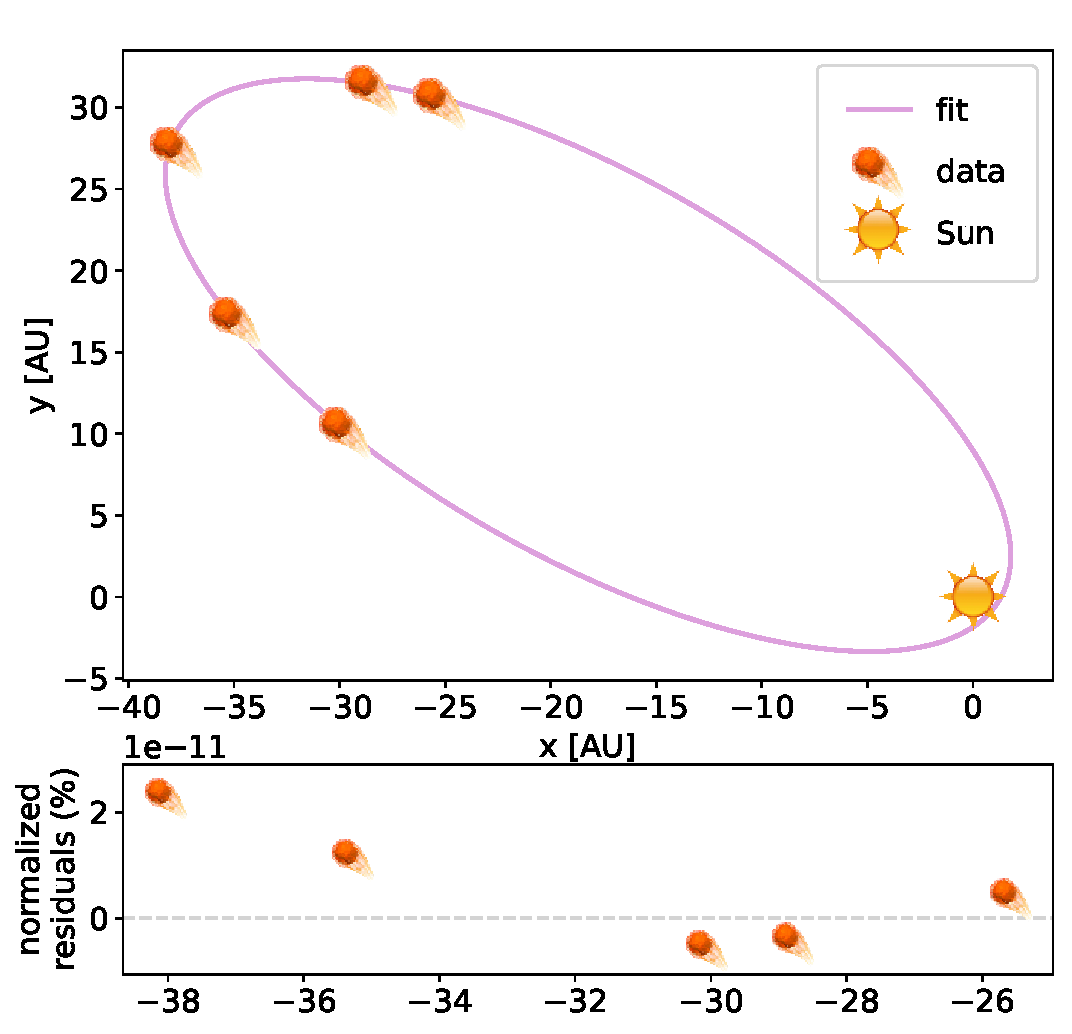
\includegraphics[width=0.5\linewidth]{Q1a.pdf}
        \caption{\label{fig:1a} Best fit ellipse and data points, with $A=-0.0357$, $B=-0.0271$, $C=-0.0465$, $D=-0.2625$, $F=0.1659$, and $G=0.7752$.}
    \end{figure}
\end{enumerate}

\item \textbf{How many computational physicists does it take to screw in a lightbulb?}
\begin{enumerate}
  \item \code{get\_etas(T, l1, l2, lN)} in \code{Lab3\_Q2.py} calculates the efficiency of a perfect blackbody (lightbulb) at temperature \code{T}, 
  for radiation between $\lambda_1=$\code{l1} and $\lambda_2=$\code{l2} using Gaussian Quadrature with \code{lN} points. The efficiency is defined as 
  \begin{align*}
    \eta &= \frac{E(\lambda_1,\lambda_2)}{E(0,\infty)},
  \end{align*}
  where 
  \begin{align}
    E(\lambda_1,\lambda_2) &= \int_{\lambda_1}^{\lambda_2} \frac{2\pi Ahc^2}{\lambda^5(e^{hc/\lambda k_bT}-1)} d\lambda
  \end{align}
  is the energy radiated between $\lambda_1$ and $\lambda_2$.
  The total energy emitted by the lightbulb, $E(0, \infty)$, can be evaluated analytically to be
  \begin{align}
    E(0, \infty) &= \frac{4Ak_b^4\pi^5T^4}{15c^2h^3}.
  \end{align} 
  The analytical expression for $E(0,\infty)$ will be used to calculate $\eta$, since the undefined integrand at $\lambda=0$ makes accurate numerical calculations impractical (Figure \ref{fig:2a} shows an accurate calculation would require more than 5000 points). 
  The area $A$ is a constant factor for all $E$, which drops out of the calculation of $\eta$ and is thus omitted from the code.
  \begin{figure}[H]
    \centering 
    \captionsetup{margin=3.2cm}
    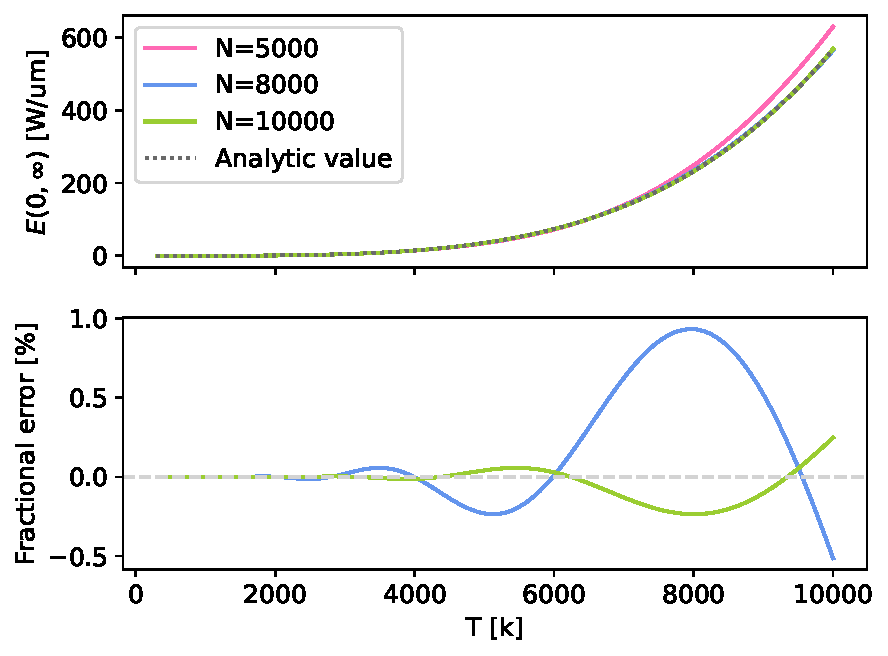
\includegraphics[width=0.48\linewidth]{Q2a.pdf}
    \caption{\label{fig:2a} $E(0,\infty)$ obtained analytically and using Gaussian Quadrature with $A=1$ m$^2$.}
    \end{figure}

  \item Using \code{ln}=70 (roughly chosen to minimize error estimates in Figure \ref{fig:2bc} c)), we plot the efficiency $\eta$ from 300 K to 10,000K in Figure \ref{fig:2bc}. 
  However, we would then also need to take the second derivative (which has a complicated expression and increases roundoff error due to added operations).
  \begin{figure}[H]
    \centering 
    \captionsetup{margin=3.2cm}
    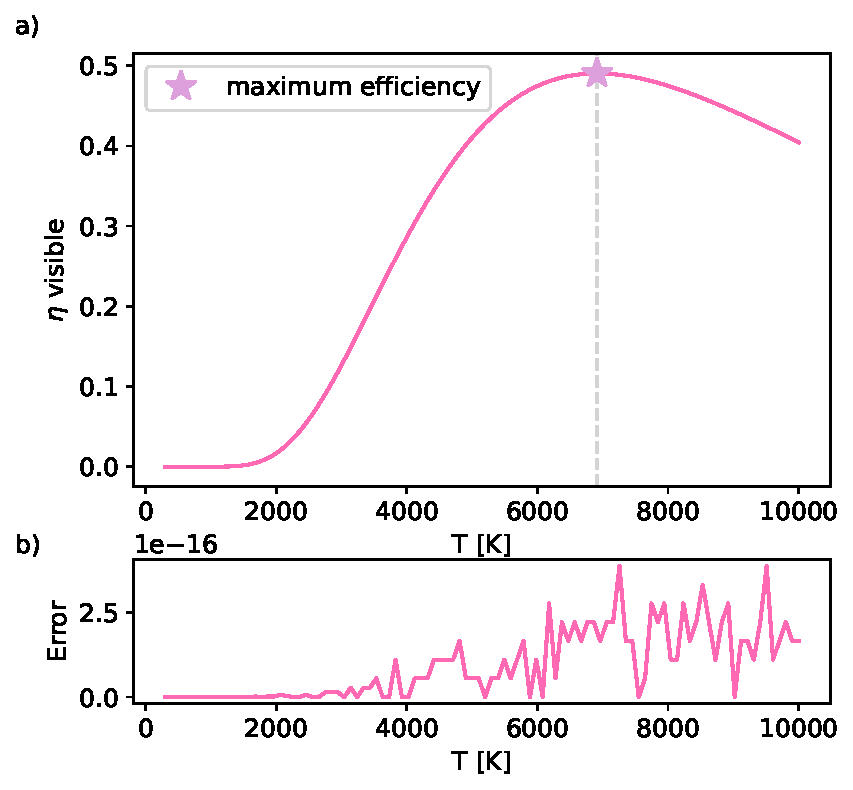
\includegraphics[width=0.5\linewidth]{Q2bc.pdf}
    \caption{\label{fig:2bc} b) $\eta$ from 300 K to 10,000K for visible (380-780 nm) radiation and c) error $\epsilon=(I_{2N} - I_N)/I_N$}
  \end{figure}
  \item Using the golden ratio method to find the temperature of maximum efficiency, we find $T_{max}=6913 K$ and $\eta_{max}=0.49$. Albeit slow, golden ratio suffices in this instance, since the majority of computational power in evaluating $\eta$ arises from finding the weights and positions for Gaussian Quadrature, which only needs to be computed once across all iterations 
  (since the integration bounds are constant)\footnote{To speed up the calculation, we could also take the first derivative of $\eta$ and search for its roots using Newton's method (Binary search is computationally equivalent to Golden Ratio, and it would be hard to isolate for $T$ in $\partial\eta(T)_T$ with which to use the Relaxation method).}
  
  \item For a lightbulb emitting in the infrared, using the same calculation procedure as in a) and c) (with \code{l1}=780 nm and \code{l2}=2250 nm), we find that the temperature of maximum efficiency is now $T_{max}=2925 K$ with $\eta_{max}=0.67$. 
  The IR efficiency from 300 to 10000 K is shown in Figure \ref{fig:2d}.
  
  \begin{figure}[h]
    \centering 
    \captionsetup{margin=3.2cm}
    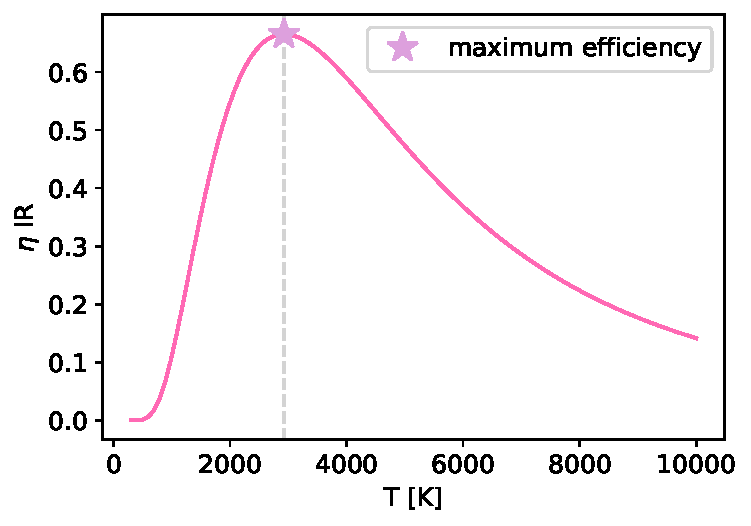
\includegraphics[width=0.5\linewidth]{Q2d.pdf}
    \caption{\label{fig:2d} $\eta$ from 300 K to 10,000K for IR (780-2250 nm) radiation.}
  \end{figure}

  The melting point of Tungsten is around 3700 K\footnote{\fullcite{blah}}, which is above the optimal temperature for $IR$ radiation, but below that of visible light. 
  It is possible to operate a light bulb at maximum efficiency in the IR region, but not for visible wavelengths.
\end{enumerate}


\end{enumerate}

\end{document}